\documentclass[12pt,border=2mm]{standalone}
\usepackage{pgfplots}
\usepgfplotslibrary{groupplots}
\pgfplotsset{compat=1.18}
\definecolor{BCred}{rgb}{0.7, 0.11, 0.11}
\definecolor{BCblue}{rgb}{0.0, 0.20, 0.42}
\pgfplotsset{every axis/.append style={
  width=7.5cm, height=7.5cm, scale only axis,
  ticklabel style={font=\small, /pgf/number format/fixed},
  yticklabel style={text width=10mm, align=right},
  ylabel style={text width=10mm, align=center},
  label style={font=\normalsize},
  title style={font=\normalsize},
  legend style={draw=none, font=\small}}}
\begin{document}
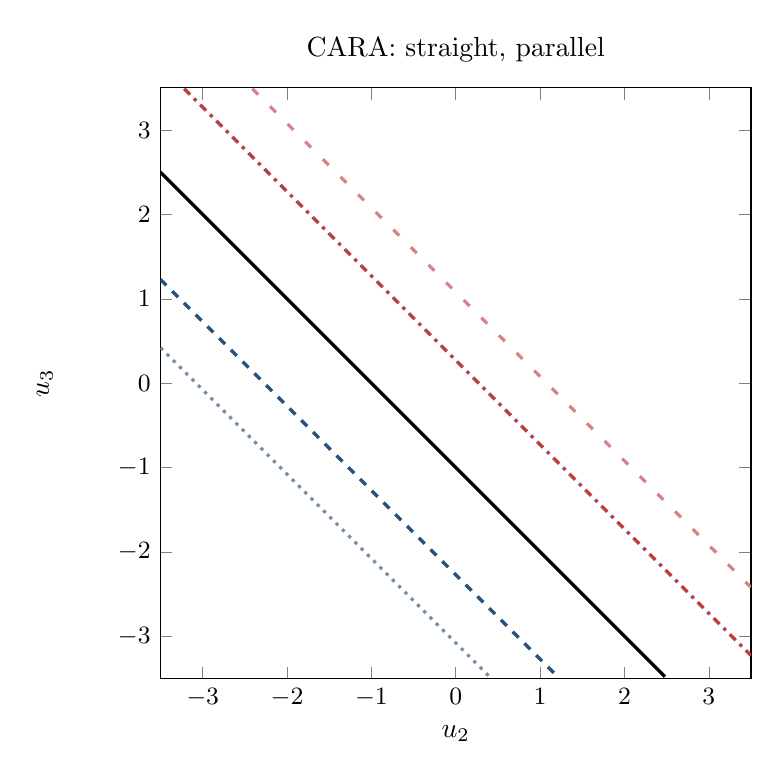
\begin{tikzpicture}
\begin{groupplot}[group style={group size=1 by 1}]
\nextgroupplot[
  xmin=-3.5, xmax=3.5, ymin=-3.5, ymax=3.5,
  xlabel={$u_2$}, ylabel={$u_3$},
  axis equal image,
  title={CARA: straight, parallel}]
% p=0.2 (real solver data — same color/dash as 3B)
\addplot[very thick,color=BCblue!55,dotted] coordinates {(-3.500,0.421)(0.405,-3.484)};
% p=0.3
\addplot[very thick,color=BCblue!85,dashed] coordinates {(-3.500,1.229)(1.214,-3.485)};
% p=0.5
\addplot[very thick,color=black] coordinates {(-3.500,2.500)(2.480,-3.480)};
% p=0.7
\addplot[very thick,color=BCred!85,dashdotted] coordinates {(-3.219,3.490)(3.500,-3.229)};
% p=0.8
\addplot[very thick,color=BCred!55,loosely dashed] coordinates {(-2.410,3.489)(3.500,-2.421)};
\end{groupplot}
\end{tikzpicture}
\end{document}
